\documentclass[aspectratio=169,11pt]{beamer}

\makeatletter
\NeedsTeXFormat{LaTeX2e}
\ProvidesPackage{beamerthemeDUNEProfessional}[2026/08/19 DUNE professional Beamer theme]

\mode<presentation>

\RequirePackage{iftex}
\RequirePackage{graphicx}
\RequirePackage{xcolor}
\RequirePackage{tikz}
\RequirePackage{adjustbox}
\RequirePackage{array}
\RequirePackage{booktabs}
\RequirePackage{tabularx}
\RequirePackage{ragged2e}

\usetikzlibrary{arrows.meta,calc,fit,positioning,shapes.geometric}

\useinnertheme{default}
\useoutertheme{default}
\usefonttheme{professionalfonts}
\setbeamertemplate{navigation symbols}{}

% Logo path is relative to a deck directory. Override with \DuneSetLogoPath.
\newcommand{\DuneLogoPath}{../../templates/dune-professional/logos}
\newcommand{\DuneSetLogoPath}[1]{\renewcommand{\DuneLogoPath}{#1}}

% Color roles. Keep semantic names in decks; avoid ad hoc local colors.
\definecolor{DuneBg}{HTML}{101820}
\definecolor{DunePanel}{HTML}{1B2733}
\definecolor{DunePanelAlt}{HTML}{263645}
\definecolor{DuneTitleBand}{HTML}{20303E}
\definecolor{DuneLine}{HTML}{536878}
\definecolor{DuneText}{HTML}{F1F5F7}
\definecolor{DuneMuted}{HTML}{BAC6CF}
\definecolor{DuneOrange}{HTML}{F2682B}
\definecolor{DuneCyan}{HTML}{8EDDF2}
\definecolor{DuneMint}{HTML}{9BD7AE}
\definecolor{DuneYellow}{HTML}{E8C85A}
\definecolor{DuneRed}{HTML}{F38B7F}
\definecolor{DuneViolet}{HTML}{B8A7E8}

\setbeamercolor{normal text}{fg=DuneText,bg=DuneBg}
\setbeamercolor{title}{fg=white,bg=DuneBg}
\setbeamercolor{subtitle}{fg=DuneMuted,bg=DuneBg}
\setbeamercolor{author}{fg=DuneCyan,bg=DuneBg}
\setbeamercolor{date}{fg=DuneMuted,bg=DuneBg}
\setbeamercolor{frametitle}{fg=white,bg=DuneBg}
\setbeamercolor{headline}{fg=DuneMuted,bg=DuneBg}
\setbeamercolor{footline}{fg=DuneMuted,bg=DuneBg}
\setbeamercolor{itemize item}{fg=DuneOrange}
\setbeamercolor{itemize subitem}{fg=DuneCyan}
\setbeamercolor{enumerate item}{fg=DuneOrange}
\setbeamercolor{caption name}{fg=DuneMuted}

\setbeamercolor{dune panel}{fg=DuneText,bg=DunePanel}
\setbeamercolor{dune panel alt}{fg=DuneText,bg=DunePanelAlt}
\setbeamercolor{dune accent}{fg=DuneBg,bg=DuneCyan}
\setbeamercolor{dune decision}{fg=DuneBg,bg=DuneYellow}
\setbeamercolor{dune risk}{fg=DuneBg,bg=DuneRed}
\setbeamercolor{dune evidence}{fg=DuneBg,bg=DuneMint}
\setbeamercolor{dune violet}{fg=DuneBg,bg=DuneViolet}

\setbeamerfont{normal text}{size=\small}
\setbeamerfont{title}{series=\bfseries}
\setbeamerfont{subtitle}{size=\large}
\setbeamerfont{author}{size=\normalsize,series=\bfseries}
\setbeamerfont{date}{size=\small}
\setbeamerfont{frametitle}{series=\bfseries}
\setbeamerfont{footline}{size=\scriptsize}

\ifPDFTeX
  \RequirePackage[scaled]{helvet}
  \renewcommand*\familydefault{\sfdefault}
  \RequirePackage[T1]{fontenc}
\else
  \RequirePackage{fontspec}
  \defaultfontfeatures{Ligatures=TeX,Scale=MatchLowercase}
  \IfFontExistsTF{IBM Plex Sans}{
    \setsansfont{IBM Plex Sans}
    \setmainfont{IBM Plex Sans}
  }{
    \IfFontExistsTF{Helvetica Neue}{
      \setsansfont{Helvetica Neue}
      \setmainfont{Helvetica Neue}
    }{
      \IfFontExistsTF{TeX Gyre Heros}{
        \setsansfont{TeX Gyre Heros}
        \setmainfont{TeX Gyre Heros}
      }{
        \IfFontExistsTF{Liberation Sans}{
          \setsansfont{Liberation Sans}
          \setmainfont{Liberation Sans}
        }{
          \setsansfont{DejaVu Sans}
          \setmainfont{DejaVu Sans}
        }
      }
    }
  }
  \IfFontExistsTF{JetBrains Mono}{
    \setmonofont{JetBrains Mono}[Scale=0.88]
  }{
    \IfFontExistsTF{Latin Modern Mono}{
      \setmonofont{Latin Modern Mono}[Scale=0.88]
    }{
      \setmonofont{DejaVu Sans Mono}[Scale=0.88]
    }
  }
  \renewcommand*\familydefault{\sfdefault}
\fi

\setbeamersize{text margin left=0.78cm,text margin right=0.78cm}
\setlength{\leftmargini}{1.15em}
\setlength{\leftmarginii}{1.05em}
\setlength{\parskip}{0.18em}

\setbeamertemplate{itemize item}{%
  \color{DuneOrange}\raisebox{0.15ex}{\scriptsize$\blacktriangleright$}%
}
\setbeamertemplate{itemize subitem}{%
  \color{DuneCyan}\raisebox{0.15ex}{\tiny$\blacktriangleright$}%
}

% Measured boxes: content may shrink down, but never expands outside the safe box.
\newcommand{\DuneFitBox}[3]{%
  \begin{adjustbox}{max width=#1,max totalheight=#2}%
    \begin{minipage}{#1}\raggedright #3\end{minipage}%
  \end{adjustbox}%
}

\newcommand{\DuneTightList}{%
  \setlength{\itemsep}{0.45mm}%
  \setlength{\parskip}{0pt}%
}

\newcommand{\DuneEyebrow}[1]{%
  {\color{DuneCyan}\scriptsize\bfseries #1\par}%
}

\newcommand{\DunePill}[2]{%
  \tikz[baseline=-0.55ex]\node[
    rounded corners=2.5pt,
    draw=#1,
    fill=#1!18!DuneBg,
    inner xsep=4pt,
    inner ysep=1.35pt,
    text=#1,
    font=\tiny\bfseries
  ]{#2};%
}

\newcommand{\DuneCard}[4][dune panel]{%
  \begin{beamercolorbox}[wd=\linewidth,sep=5pt,rounded=true]{#1}
    {\usebeamercolor[fg]{#1}\bfseries #2\par}
    \vspace{0.4mm}
    {\usebeamercolor[fg]{#1}\footnotesize #3\par}
    \if\relax\detokenize{#4}\relax\else
      \vspace{0.5mm}{\usebeamercolor[fg]{#1}\scriptsize #4\par}
    \fi
  \end{beamercolorbox}
}

\newcommand{\DuneFixedCard}[5][dune panel]{%
  \begin{beamercolorbox}[wd=\linewidth,sep=5pt,rounded=true]{#1}
    \begin{minipage}[t][#2][t]{\dimexpr\linewidth-10pt\relax}
      \raggedright
      {\usebeamercolor[fg]{#1}\bfseries #3\par}
      \vspace{0.45mm}
      {\usebeamercolor[fg]{#1}\footnotesize #4\par}
      \if\relax\detokenize{#5}\relax\else
        \vspace{0.55mm}{\usebeamercolor[fg]{#1}\scriptsize #5\par}
      \fi
    \end{minipage}
  \end{beamercolorbox}
}

\newcommand{\DuneFooterLogo}{%
  \IfFileExists{\DuneLogoPath/logosolo.png}{%
    \tikz[baseline=-0.52ex]\node[opacity=0.42,inner sep=0pt]{%
      \includegraphics[height=0.25cm]{\DuneLogoPath/logosolo.png}%
    };%
  }{}%
}

\newcommand{\DuneTalkDate}{%
  \@ifundefined{mydate}{\today}{\mydate}%
}

% Background and fixed frame-title band.
\addtobeamertemplate{background canvas}{%
  \begin{tikzpicture}[remember picture,overlay]
    \fill[DuneBg] (current page.south west) rectangle (current page.north east);
    \draw[DuneLine,line width=0.55pt]
      ($(current page.south west)+(0.78,0.74)$)
      -- ($(current page.south east)+(-0.78,0.74)$);
    \fill[DuneCyan!16]
      ($(current page.south east)+(-3.2,0.83)$) rectangle ++(1.45,0.055);
  \end{tikzpicture}%
}{}

\setbeamertemplate{headline}{}

\setbeamertemplate{frametitle}{%
  \nointerlineskip%
  \begin{tikzpicture}[remember picture,overlay]
    \fill[DuneTitleBand]
      (current page.north west) rectangle ($(current page.north east)+(0,-1.18)$);
    \fill[DuneOrange]
      ($(current page.north west)+(0.78,-0.23)$) rectangle ++(1.38,0.055);
    \node[anchor=west,inner sep=0pt]
      at ($(current page.north west)+(0.78,-0.72)$) {%
        \DuneFitBox{\dimexpr\paperwidth-1.56cm\relax}{6.7mm}{%
          {\color{white}\bfseries\fontsize{17}{20}\selectfont\insertframetitle}%
        }%
      };
    \ifx\insertframesubtitle\@empty\else
      \node[anchor=west,inner sep=0pt]
        at ($(current page.north west)+(0.78,-1.02)$) {%
          \DuneFitBox{\dimexpr\paperwidth-1.56cm\relax}{3.2mm}{%
            {\color{DuneMuted}\scriptsize\insertframesubtitle}%
          }%
        };
    \fi
  \end{tikzpicture}%
  \vspace*{12.5mm}%
}

\setbeamertemplate{footline}{%
  \leavevmode%
  \begin{beamercolorbox}[wd=\paperwidth,ht=6.4mm,dp=1.8mm,leftskip=0.78cm,rightskip=0.78cm]{footline}
    \DuneFooterLogo\hspace{0.45em}{\textcolor{DuneMuted}{\DuneTalkDate}}%
    \hfill%
    {\textcolor{DuneOrange}{\bfseries\insertframenumber}\textcolor{DuneMuted}{/\inserttotalframenumber}}%
  \end{beamercolorbox}%
}

\setbeamertemplate{title page}{%
  \begin{tikzpicture}[remember picture,overlay]
    \fill[DuneBg] (current page.south west) rectangle (current page.north east);
    \fill[DuneTitleBand]
      (current page.north west) rectangle ($(current page.north east)+(0,-3.03)$);
    \fill[DuneOrange]
      ($(current page.north west)+(0.82,-0.58)$) rectangle ++(1.55,0.075);
    \fill[DuneCyan]
      ($(current page.south east)+(-2.8,0.79)$) rectangle ++(1.88,0.065);
    \IfFileExists{\DuneLogoPath/DUNElogo_white.png}{%
      \node[anchor=south east,opacity=0.13,inner sep=0pt]
        at ($(current page.south east)+(-0.55,1.42)$) {%
        \includegraphics[width=0.34\paperwidth]{\DuneLogoPath/DUNElogo_white.png}%
      };
    }{}%
    \IfFileExists{\DuneLogoPath/FNAL-Logo-NAL-Light.png}{%
      \node[anchor=south east,inner sep=0pt]
        at ($(current page.south east)+(-0.92,0.78)$) {%
        \includegraphics[height=0.42cm]{\DuneLogoPath/FNAL-Logo-NAL-Light.png}%
      };
    }{}%
    \node[anchor=north west,inner sep=0pt]
      at ($(current page.north west)+(0.82,-0.88)$) {%
        \DuneFitBox{0.78\paperwidth}{1.48cm}{%
          {\color{white}\bfseries\fontsize{25}{28}\selectfont\inserttitle}%
        }%
      };
    \node[anchor=north west,inner sep=0pt]
      at ($(current page.north west)+(0.82,-3.55)$) {%
        \DuneFitBox{0.56\paperwidth}{1.35cm}{%
          {\color{DuneMuted}\fontsize{13}{17}\selectfont\insertsubtitle}%
        }%
      };
    \node[anchor=north west,text=DuneCyan,font=\bfseries,inner sep=0pt]
      at ($(current page.north west)+(0.82,-6.3)$) {\insertauthor};
    \node[anchor=north west,text=DuneMuted,font=\small,inner sep=0pt]
      at ($(current page.north west)+(0.82,-6.82)$) {\insertdate};
  \end{tikzpicture}%
  \vfill%
}

\tikzset{
  dune repo/.style={
    draw=DuneCyan,
    fill=DuneCyan!12!DunePanel,
    text=DuneText,
    rounded corners=3pt,
    align=center,
    text width=2.35cm,
    minimum height=0.86cm,
    inner sep=4pt,
    font=\scriptsize\bfseries
  },
  dune repo muted/.style={
    draw=DuneLine,
    fill=DunePanelAlt,
    text=DuneText,
    rounded corners=3pt,
    align=center,
    text width=2.35cm,
    minimum height=0.86cm,
    inner sep=4pt,
    font=\scriptsize\bfseries
  },
  dune artifact/.style={
    draw=DuneMint,
    fill=DuneMint!13!DunePanel,
    text=DuneText,
    rounded corners=3pt,
    align=center,
    text width=2.35cm,
    minimum height=0.86cm,
    inner sep=4pt,
    font=\scriptsize\bfseries
  },
  dune decision node/.style={
    draw=DuneYellow,
    fill=DuneYellow!14!DunePanel,
    text=DuneText,
    rounded corners=3pt,
    align=center,
    text width=2.35cm,
    minimum height=0.86cm,
    inner sep=4pt,
    font=\scriptsize\bfseries
  },
  dune flow/.style={-Latex,draw=DuneCyan,line width=0.85pt},
  dune relation/.style={draw=DuneMuted,line width=0.65pt},
  dune evidence flow/.style={-Latex,draw=DuneViolet,dashed,line width=0.85pt},
  dune label/.style={
    fill=DuneBg,
    text=DuneMuted,
    inner sep=1.5pt,
    font=\tiny,
    align=center
  }
}

\mode<all>

\makeatother

\usepackage{booktabs}
\usepackage{siunitx}
\usepackage{tikz}
\usetikzlibrary{arrows.meta,positioning,fit}

\title{PDS channel activity meets firmware dead time}
\subtitle{Matched FD-VD/FD-HD LArSoft results and a 1024-versus-512 trace replay}
\author{Manuel Arroyave}
\date{PDS discussion -- September 2026}
\newcommand{\mydate}{September 2026}
\hypersetup{colorlinks=true,urlcolor=DuneInfo,linkcolor=DuneInfo}

\newcommand{\simrepo}{\texttt{daphne\_mezz\_xc\_sim}}
\newcommand{\oldplots}{../../../daphne/firmware/repos/daphne_mezz_xc_sim/data/output/plots}

% Deck-local geometry corrections. Keep these out of the shared theme so other
% presentations retain their reviewed layouts.
\setbeamertemplate{title page}{%
  \begin{tikzpicture}[remember picture,overlay]
    \fill[DuneBackground] (current page.south west) rectangle (current page.north east);
    \fill[DuneTitleSurface]
      (current page.north west) rectangle ($(current page.north east)+(0,-3.03)$);
    \fill[DunePrimary]
      ($(current page.north west)+(0.82,-0.58)$) rectangle ++(1.55,0.075);
    \fill[DuneSky]
      ($(current page.south east)+(-2.8,0.79)$) rectangle ++(1.88,0.065);
    \IfFileExists{\DuneLogoPath/DUNElogo_white.png}{%
      \node[anchor=south east,opacity=0.13,inner sep=0pt]
        at ($(current page.south east)+(-0.55,1.42)$) {%
        \includegraphics[width=0.34\paperwidth]{\DuneLogoPath/DUNElogo_white.png}%
      };
    }{}%
    \IfFileExists{\DuneLogoPath/FNAL-Logo-NAL-Light.png}{%
      \node[anchor=south east,inner sep=0pt]
        at ($(current page.south east)+(-0.92,1.08)$) {%
        \includegraphics[height=0.42cm]{\DuneLogoPath/FNAL-Logo-NAL-Light.png}%
      };
    }{}%
    \node[anchor=north west,inner sep=0pt]
      at ($(current page.north west)+(0.82,-0.88)$) {%
        \DuneFitBox{0.78\paperwidth}{1.48cm}{%
          {\color{DuneText}\bfseries\fontsize{25}{28}\selectfont\inserttitle}%
        }%
      };
    \node[anchor=north west,inner sep=0pt]
      at ($(current page.north west)+(0.82,-3.55)$) {%
        \DuneFitBox{0.56\paperwidth}{1.35cm}{%
          {\color{DuneTextMuted}\fontsize{13}{17}\selectfont\insertsubtitle}%
        }%
      };
    \node[anchor=north west,text=DuneSky,font=\bfseries,inner sep=0pt]
      at ($(current page.north west)+(0.82,-6.3)$) {\insertauthor};
    \node[anchor=north west,text=DuneTextMuted,font=\small,inner sep=0pt]
      at ($(current page.north west)+(0.82,-6.82)$) {\insertdate};
  \end{tikzpicture}%
  \vfill%
}

\renewcommand{\DuneSectionPage}[3]{%
  \begin{frame}[plain]
    \begin{tikzpicture}[remember picture,overlay]
      \fill[DuneTitleSurface] (current page.south west) rectangle (current page.north east);
      \fill[DunePrimary]
        ($(current page.north west)+(0.88,-0.62)$) rectangle ++(1.75,0.085);
      \fill[DuneSky!9!DuneTitleSurface]
        ($(current page.north east)+(-4.15,0)$) rectangle (current page.south east);
      \draw[DuneBorder,line width=0.75pt]
        ($(current page.south west)+(0.88,0.72)$)
        -- ($(current page.south east)+(-0.88,0.72)$);
      \fill[DuneSky]
        ($(current page.south east)+(-2.9,0.54)$) rectangle ++(1.95,0.075);
      \node[anchor=north west,text=DuneSky,font=\footnotesize\bfseries,inner sep=0pt]
        at ($(current page.north west)+(0.88,-1.02)$) {#1};
      \node[anchor=north west,text=DuneText,font=\bfseries,align=left,text width=0.67\paperwidth,inner sep=0pt]
        at ($(current page.north west)+(0.88,-2.30)$)
        {\fontsize{27}{31}\selectfont #2};
      \node[anchor=south west,text=DuneTextMuted,align=left,text width=0.69\paperwidth,inner sep=0pt]
        at ($(current page.south west)+(0.88,1.10)$)
        {\fontsize{12.5}{16}\selectfont #3};
    \end{tikzpicture}
  \end{frame}%
}

\begin{document}

\begin{frame}[plain]
  \titlepage
\end{frame}

\begin{frame}{The simulation now connects activity to channel busy time}
  \begin{columns}[T,onlytextwidth]
    \begin{column}{0.59\textwidth}
      \DuneBigStatement{CURRENT READING}
        {VD cathode channels are 3.6--4.3 times busier before firmware loss.}
        {Replaying the actual candidate times through the fixed-record busy gate shows that 512 samples recovers activity in both technologies, especially VD.}
    \end{column}
    \begin{column}{0.37\textwidth}
      \DuneCompactNumberBlock{paper}{01}{Input activity}
        {Eight shards per detector and source at a matched 0.7-PE threshold.}
      \smallskip
      \DuneCompactNumberBlock{sky}{02}{Coupled result}
        {Actual per-channel times drive the XC fixed-record busy gate.}
      \smallskip
      \DuneCompactNumberBlock{coral}{03}{Still missing}
        {Continuous ADC, full XC/CFD, transport, noise, and containment.}
    \end{column}
  \end{columns}
\end{frame}

\DuneSectionPage{WHY THIS MATTERS}{Dead time is not only a throughput metric}
  {It changes which optical signatures survive long enough to become trigger evidence.}

\begin{frame}{Low-energy and non-beam signatures stress the readout differently}
  \begin{columns}[T,onlytextwidth]
    \begin{column}{0.48\textwidth}
      \DuneFixedColorBlock{paper}{3.18cm}{LOCAL, BRIGHT, OR PROMPT}{One interaction is visible}
        {A localized flash gives a time anchor. Peak, integral, width, and multiplicity describe it; nearby activity may still overlap the busy window.}
    \end{column}
    \begin{column}{0.48\textwidth}
      \DuneFixedColorBlock{sky}{3.18cm}{LOW-LIGHT OR DISTRIBUTED}{The pattern carries the evidence}
        {A supernova-like signal is a detector-wide rate excess. Near threshold, stable baselines and noise rejection protect many modest observations.}
    \end{column}
  \end{columns}

  \smallskip
  \DuneCompactColorBlock{coral}{COMMON FAILURE MODE}{Dead time removes evidence before DAQ can combine it}
    {A lost waveform is not merely fewer bytes: it can bias local multiplicity, distort time structure, or suppress the rate excess used by a downstream non-beam trigger.}
\end{frame}

\begin{frame}{Local signatures depend on pulse-level evidence}
  \footnotesize
  \setlength{\tabcolsep}{2pt}
  \renewcommand{\arraystretch}{1.22}
  \begin{tabular}{@{}p{0.19\textwidth}p{0.25\textwidth}p{0.25\textwidth}p{0.25\textwidth}@{}}
    \toprule
    Signature & Expected optical pattern & Preserve & Dead-time sensitivity \\
    \midrule
    Prompt energetic interaction & Bright, localized flash across nearby channels; ns--\(\mu\)s & leading time, peak, integral, width, saturation, multiplicity & nearby or delayed activity can fall inside the active window \\
    Low-energy isolated interaction & Few-PE evidence across one or several channels; ns--\(\mu\)s & near-threshold efficiency, timing, charge, coincidence & one lost pulse can break a coincidence or cross a threshold \\
    Delayed activity & Secondary pulse or cluster after prompt light; \(\mu\)s--ms & separation, second-pulse efficiency, peak count, total light & the second component can arrive while the channel is busy \\
    \bottomrule
  \end{tabular}

  \medskip
  \DuneCompactColorBlock{paper}{LOCAL QUESTION}{What survives around one accepted trigger?}
    {These signatures test amplitude response, waveform containment, retrigger spacing, and the interpretation of nearby pulses.}
\end{frame}

\begin{frame}{Distributed signatures depend on rate and topology}
  \footnotesize
  \setlength{\tabcolsep}{2pt}
  \renewcommand{\arraystretch}{1.22}
  \begin{tabular}{@{}p{0.19\textwidth}p{0.25\textwidth}p{0.25\textwidth}p{0.25\textwidth}@{}}
    \toprule
    Signature & Expected optical pattern & Preserve & Dead-time sensitivity \\
    \midrule
    Supernova-like burst & Detector-wide rate excess of modest interactions; ms--s & rate, timing distribution, multiplicity, live time & rate-dependent losses can distort the burst excess \\
    Nucleon-decay-like candidate & Prompt light with possible delayed components; ns--ms & prompt time, delayed evidence, coincidence structure & losses may remove the delayed or lower-amplitude component \\
    Background and noise & Dark counts, radiological activity, correlated noise, afterpulses; ns--s & baseline, quality flags, classification, retrigger behavior & background creates dead time and time-dependent signal efficiency \\
    \bottomrule
  \end{tabular}

  \medskip
  \DuneCompactColorBlock{sky}{DETECTOR QUESTION}{What pattern reaches the downstream trigger?}
    {These signatures test whether channel-level losses bias multi-channel rates, coincidences, and long-window structure.}
\end{frame}

\begin{frame}{One channel recognizes a pulse; the detector recognizes a signature}
  \centering
  \begin{tikzpicture}[
    node distance=7mm and 7mm,
    box/.style={rounded corners=2pt,minimum height=1.25cm,text width=2.45cm,align=center,font=\small\bfseries,draw=none},
    flow/.style={-{Latex[length=2.4mm]},line width=1.5pt,color=DuneSky}
  ]
    \node[box,fill=DunePaper,text=DuneOnAccent] (lar) {Light in LAr\\pulse or rate pattern};
    \node[box,fill=DuneSky,text=DuneOnAccent,right=of lar] (xc) {XC self-trigger\\channel decision};
    \node[box,fill=DuneSky,text=DuneOnAccent,right=of xc] (desc) {Waveform +\\descriptors};
    \node[box,fill=DunePrimary,text=DuneOnAccent,right=of desc] (daq) {DAQ trigger\\multi-channel decision};
    \draw[flow] (lar) -- (xc);
    \draw[flow] (xc) -- (desc);
    \draw[flow] (desc) -- (daq);
    \node[below=7mm of xc,align=center,text=DuneMuted,font=\small] {Firmware can reject here\\because the channel is busy};
    \draw[-{Latex[length=2mm]},line width=1.2pt,color=DuneDanger] ([yshift=-1mm]xc.south) -- ++(0,-5mm);
  \end{tikzpicture}

  \vspace{3mm}
  \DuneDiagramCaption{The board exports local evidence. Detector-scale low-energy and non-beam decisions require DAQ to combine that evidence across channels, boards, and time windows.}
\end{frame}

\DuneSectionPage{WHAT THE EMULATOR REPRESENTS}{The simulation is already useful—but its claims have boundaries}
  {Separate waveform response, architecture dead time, and HDL signoff so one result is never asked to prove all three.}

\begin{frame}{The XC emulator follows the important DAPHNE trigger stages}
  \begin{columns}[T,onlytextwidth]
    \begin{column}{0.235\textwidth}
      \DuneCompactNumberBlock{paper}{01}{Condition}
        {Baseline filtering and the configured pulse polarity prepare ADC samples.}
    \end{column}
    \begin{column}{0.235\textwidth}
      \DuneCompactNumberBlock{sky}{02}{Recognize}
        {A 32-tap matched filter and two-cycle threshold crossing create the trigger.}
    \end{column}
    \begin{column}{0.235\textwidth}
      \DuneCompactNumberBlock{sky}{03}{Describe}
        {CFD gating and CIEMAT logic produce timing, peak, integral, width, and peak count.}
    \end{column}
    \begin{column}{0.235\textwidth}
      \DuneCompactNumberBlock{coral}{04}{Admit}
        {Builder, queue, ring, serializer, and output state determine whether a trigger survives.}
    \end{column}
  \end{columns}

  \smallskip
  \DuneCompactColorBlock{paper}{IMPLEMENTATION STATUS}{Two complementary models are in the repository}
    {\texttt{st\_xc\_sim} replays waveform-level self-trigger behavior. \texttt{ring\_deadtime\_sim} scans architecture choices quickly; sparse HDL tests remain the signoff reference.}
\end{frame}

\begin{frame}{Each simulation answers a different question}
  \begin{columns}[T,onlytextwidth]
    \begin{column}{0.48\textwidth}
      \DuneFixedColorBlock{sky}{3.18cm}{WAVEFORM REPLAY}{Will this pulse trigger and what is recorded?}
        {Uses ADC samples, RTL-aligned XC settings, descriptors, and a selected frame length. It exposes threshold response, timing, truncation, and busy-window loss.}
    \end{column}
    \begin{column}{0.48\textwidth}
      \DuneFixedColorBlock{paper}{3.18cm}{ARCHITECTURE SWEEP}{How does dead time scale with rate?}
        {Uses stochastic arrivals plus admission, queue, ring, serializer, and FIFO state. It compares rates cheaply, but contains no photon physics or event topology.}
    \end{column}
  \end{columns}

  \smallskip
  \DuneCompactColorBlock{coral}{SIGNOFF BOUNDARY}{HDL spot checks connect the two}
    {Overlay selected HDL points on the dense C++ curves. Do not label a C++ architecture sweep as firmware validation until those points agree within an accepted tolerance.}
\end{frame}

\DuneSectionPage{WHAT LARSOFT SAYS}{One VD cathode channel is several times busier than one HD channel}
  {The comparison holds threshold, waveform model, source category, and hardware-channel denominator fixed.}

\begin{frame}{Before firmware loss, VD cathode channels are 3.6--4.3 times busier}
  \begin{columns}[T,onlytextwidth]
    \begin{column}{0.66\textwidth}
      \centering
      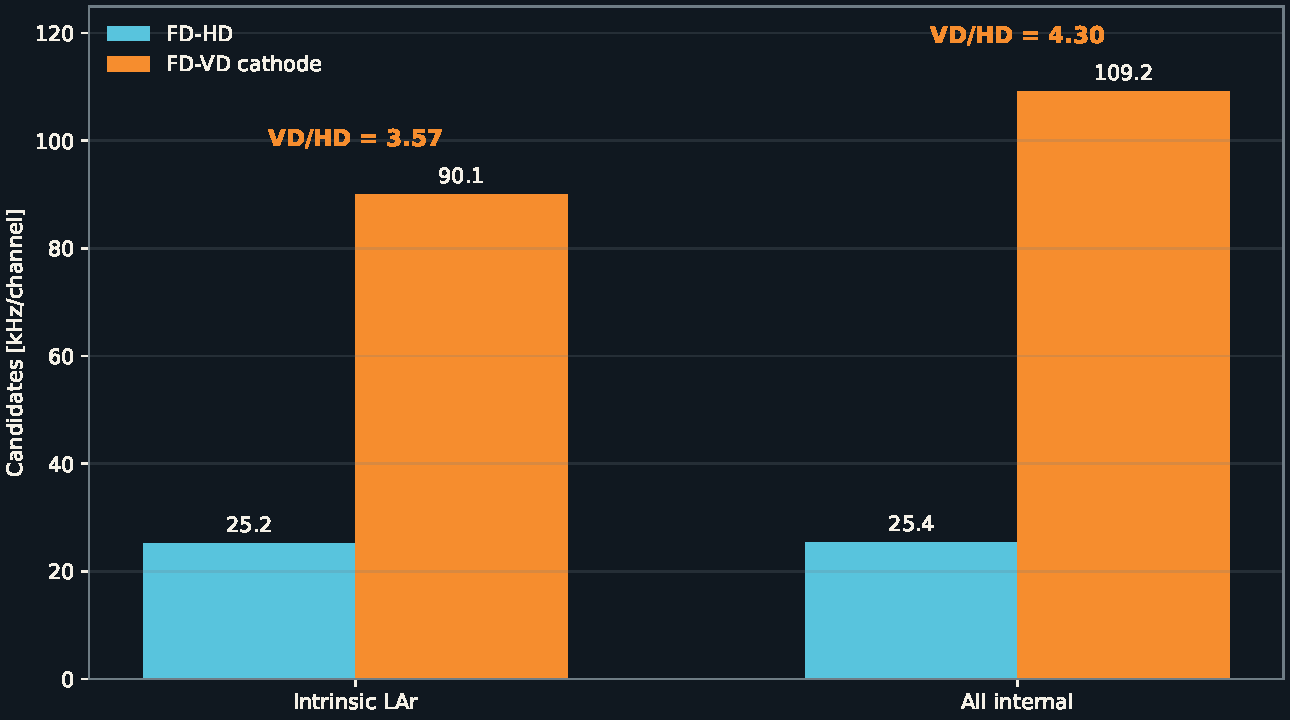
\includegraphics[width=\linewidth,height=0.55\textheight,keepaspectratio]{figures/larsoft_activity_comparison.pdf}
    \end{column}
    \begin{column}{0.30\textwidth}
      \DuneCompactNumberBlock{paper}{3.57}{Intrinsic LAr}
        {VD cathode / HD per channel.}
      \smallskip
      \DuneCompactNumberBlock{sky}{4.30}{All internal}
        {Intrinsic plus detector materials.}
      \smallskip
      \DuneCompactColorBlock{coral}{NOT A GAIN FACTOR}{Raw channel activity}
        {No area correction or firmware loss.}
    \end{column}
  \end{columns}
  \DuneDiagramCaption{Matched 0.7 PE; eight shards/source; complete 6,000-channel HD and 640-channel VD-cathode denominators.}
\end{frame}

\begin{frame}{The earlier 2025 study points in the same direction}
  \footnotesize
  \begin{tabular}{@{}p{0.24\textwidth}p{0.21\textwidth}p{0.21\textwidth}p{0.23\textwidth}@{}}
    \toprule
    Comparison & May 2025 slides & This campaign & Reading \\
    \midrule
    Intrinsic/internal light & roughly 4--5 times higher in VD & 3.57--4.30 & same several-times-busier scale \\
    External gammas & roughly 20 times higher in VD & not included & boundary model still needed \\
    Absolute rate & optical hits above 15 ADC & episodes above 0.7 PE & not directly comparable \\
    Channel population & reduced; VD classes mixed & full; VD classes separate & denominators differ \\
    \bottomrule
  \end{tabular}

  \medskip
  \DuneCompactColorBlock{paper}{BOTTOM LINE}{There is no single factor of ten}
    {The source-specific ratios span several to tens. For internal backgrounds, both studies support a VD/HD per-channel ratio of order four.}

  {\color{DuneTextMuted}Source: P. Barham Alzás, ``Hits and clusters,'' slides 4, 6--7, May 2025.\par}
\end{frame}

\begin{frame}{The new coupling uses real time structure on every channel}
  \begin{columns}[T,onlytextwidth]
    \begin{column}{0.235\textwidth}
      \DuneCompactNumberBlock{paper}{01}{LArSoft}
        {Generate light and extract 0.7-PE threshold-candidate times.}
    \end{column}
    \begin{column}{0.235\textwidth}
      \DuneCompactNumberBlock{sky}{02}{Partition}
        {Reset state independently for each event and hardware channel.}
    \end{column}
    \begin{column}{0.235\textwidth}
      \DuneCompactNumberBlock{sky}{03}{Replay}
        {Apply the XC legacy fixed-record gate to the same ordered timestamps.}
    \end{column}
    \begin{column}{0.235\textwidth}
      \DuneCompactNumberBlock{coral}{04}{Compare}
        {Use 1037 busy cycles for 1024 and 525 cycles for 512.}
    \end{column}
  \end{columns}

  \smallskip
  \DuneCompactColorBlock{paper}{EXACTLY WHAT THIS ADDS}{Candidate-level firmware acceptance}
    {The replay preserves burstiness and cross-channel event timing while maintaining independent channel state. It does not rerun the 32-tap XC filter or CFD because continuous ADC streams were not saved.}
\end{frame}

\begin{frame}{One pinned measured shape controls the electronics comparison}
  \begin{columns}[T,onlytextwidth]
    \begin{column}{0.64\textwidth}
      \centering
      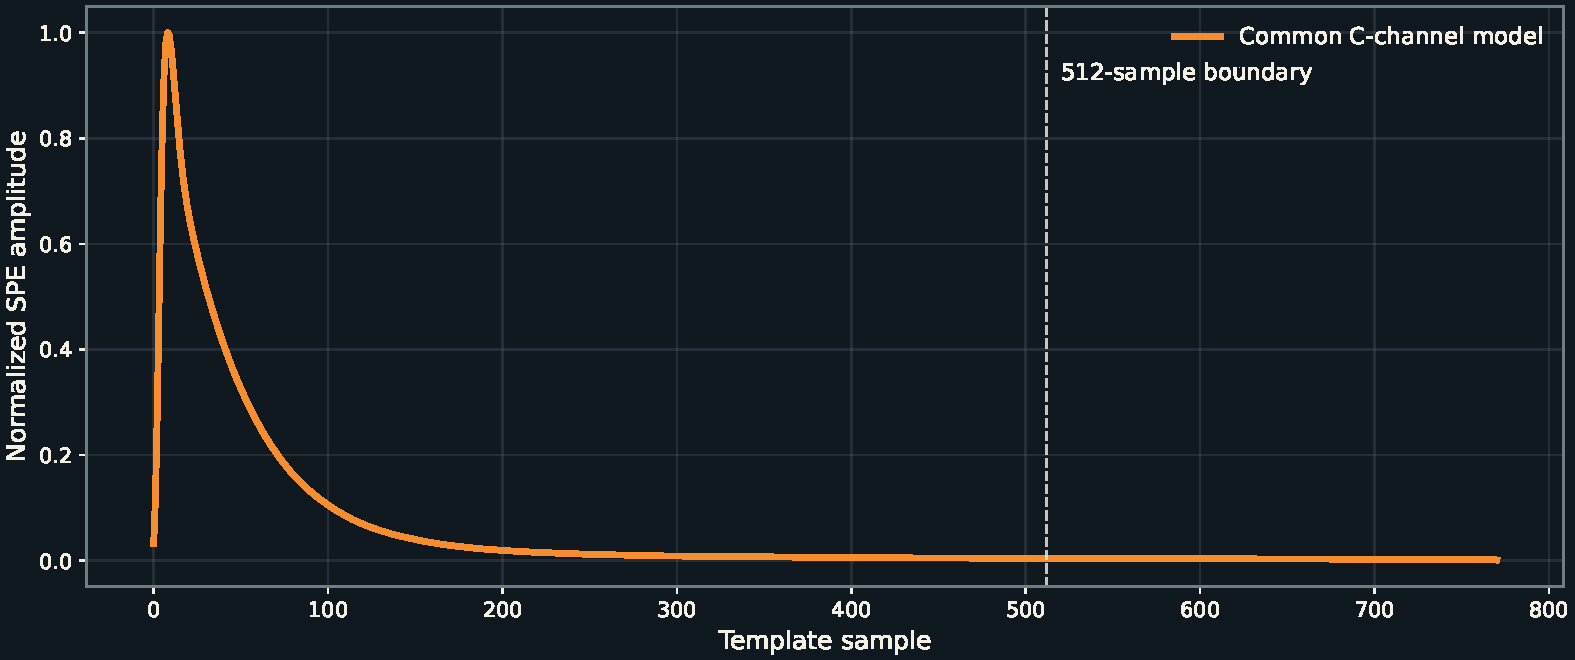
\includegraphics[width=\linewidth,height=0.48\textheight,keepaspectratio]{figures/waffles_common_c_template.pdf}
    \end{column}
    \begin{column}{0.32\textwidth}
      \DuneCompactColorBlock{paper}{SOURCE}{16 Waffles cathode C channels}
        {Large-pulse, zero-subtracted NP02 waveforms at commit \texttt{6e6274d}.}
      \smallskip
      \DuneCompactColorBlock{coral}{CONTROLLED USE}{One temporary common model}
        {The aligned mean is used for both HD and VD; it is a shape model, not an FD calibration.}
    \end{column}
  \end{columns}
  \DuneDiagramCaption{771 samples at 16 ns; 10 ADC/PE peak; the same strict $>7$-ADC threshold in HD and VD.}
\end{frame}

\DuneSectionPage{THE PRESENT BOTTLENECK}{A captured waveform keeps one channel busy}
  {The 1024-sample format protects context, but it also suppresses triggers that arrive while the builder is occupied.}

\begin{frame}{Shortening the record attacks the longest first-order busy interval}
  \centering
  \begin{tikzpicture}[x=0.105cm,y=0.82cm]
    \fill[DunePaper] (0,1.35) rectangle (102.4,2.05);
    \fill[DunePrimary] (0,0.10) rectangle (51.2,0.80);
    \draw[DuneMuted,line width=1pt] (51.2,-0.05) -- (51.2,2.2);
    \node[anchor=west,text=DuneOnAccent,font=\bfseries] at (2,1.70) {1024 samples: longer channel occupancy};
    \node[anchor=west,text=DuneOnAccent,font=\small\bfseries] at (2,0.45) {512 samples: shorter occupancy};
    \node[anchor=south,text=DuneMuted,font=\small] at (51.2,2.22) {512 samples};
    \draw[-{Latex[length=2.5mm]},line width=1.4pt,color=DuneDanger] (74,2.4) -- (74,2.08);
    \node[anchor=south,align=center,text=DuneDanger,font=\small\bfseries] at (74,2.42) {a new trigger here is rejected\\by the legacy busy path};
  \end{tikzpicture}

  \DuneDiagramCaption{Halving the fixed record roughly halves the first-order builder occupancy; shared transport and admission rules still matter.}

  \vspace{1mm}
  \begin{columns}[T,onlytextwidth]
    \begin{column}{0.48\textwidth}
      \DuneCompactColorBlock{paper}{LEGACY MODEL}{1024 samples}
        {About 1037 busy cycles and 232 output words per accepted trigger.}
    \end{column}
    \begin{column}{0.48\textwidth}
      \DuneCompactColorBlock{coral}{FIRST MITIGATION}{512 samples}
        {About 525 busy cycles and 120 output words, while retaining the existing fixed-record concept.}
    \end{column}
  \end{columns}
\end{frame}

\begin{frame}{The model says 512 samples is the largest single practical gain}
  \begin{columns}[T,onlytextwidth]
    \begin{column}{0.67\textwidth}
      \centering
      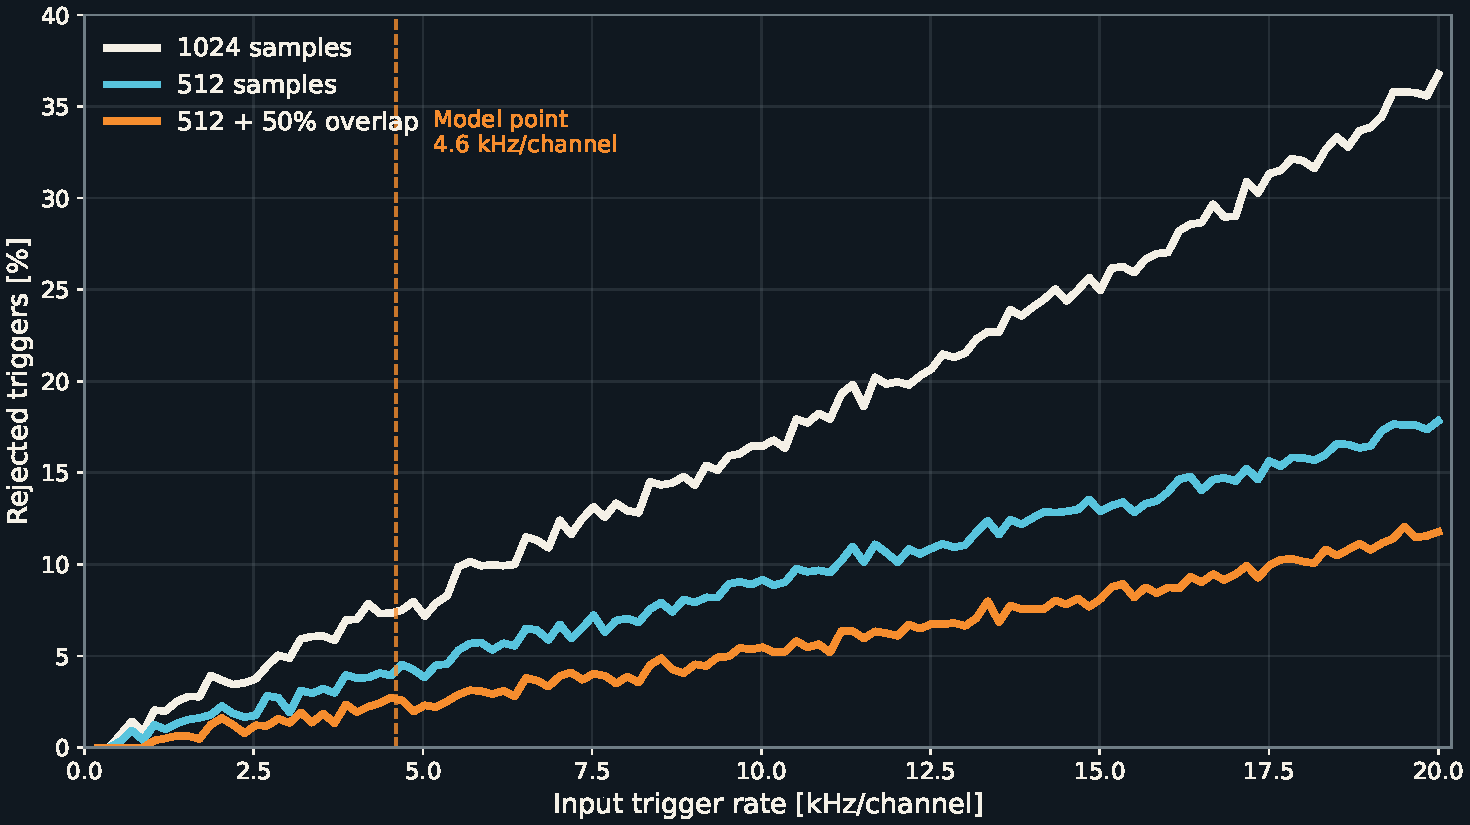
\includegraphics[width=\linewidth,height=0.60\textheight,keepaspectratio]{figures/deadtime_1024_512_ring50.pdf}
    \end{column}
    \begin{column}{0.29\textwidth}
      \DuneCompactNumberBlock{paper}{4.6k}{Model point}
        {Architecture point: modeled dead time falls from 7.41\% to 4.20\%.}
      \smallskip
      \DuneCompactNumberBlock{sky}{10k}{Stress point}
        {16.46\% becomes 9.14\% with plain 512.}
    \end{column}
  \end{columns}
  \DuneDiagramCaption{Independent-Poisson sweep: at 20 kHz/ch, 36.76\% becomes 17.83\%. The 4.6-kHz marker is a model coordinate, not a measured detector rate.}
\end{frame}

\begin{frame}{512 improves acceptance on actual LArSoft timing}
  \begin{columns}[T,onlytextwidth]
    \begin{column}{0.67\textwidth}
      \centering
      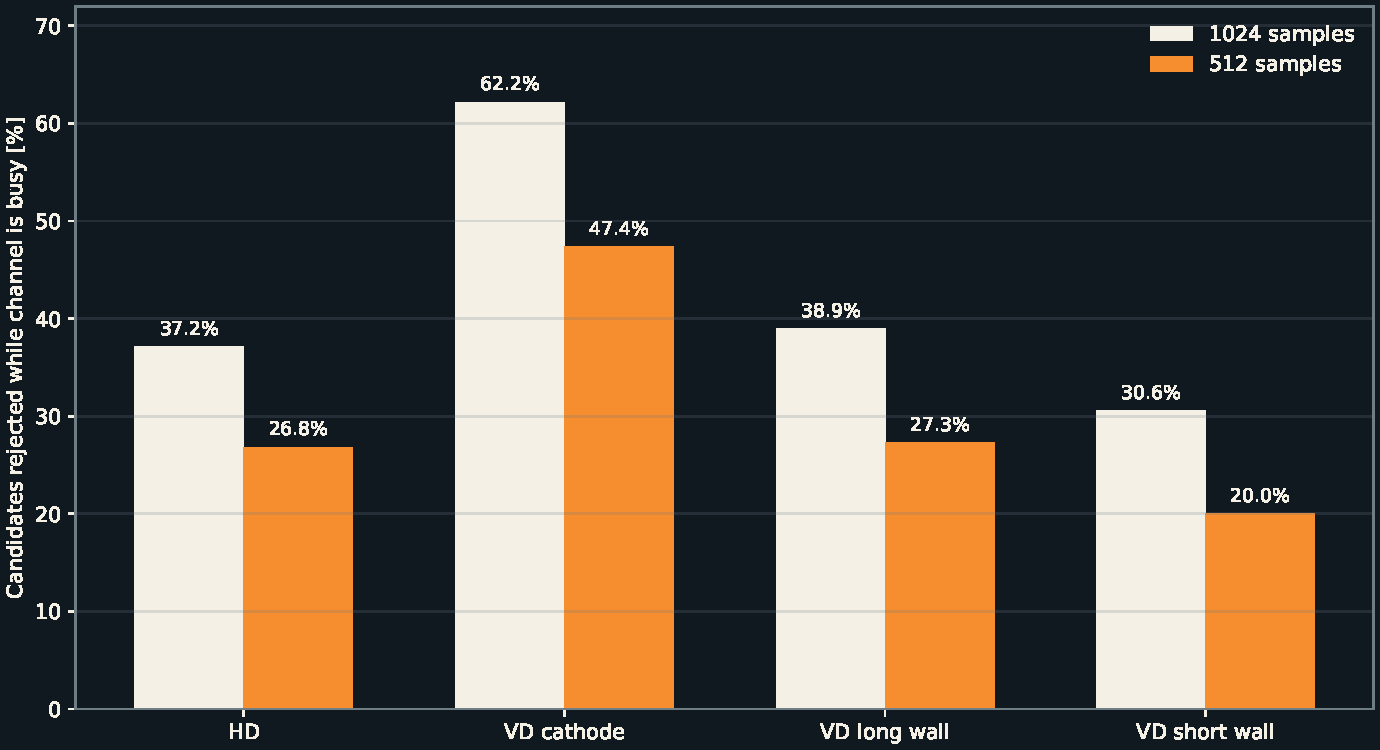
\includegraphics[width=\linewidth,height=0.49\textheight,keepaspectratio]{figures/larsoft_trace_deadtime.pdf}
    \end{column}
    \begin{column}{0.29\textwidth}
      \DuneCompactNumberBlock{paper}{HD}{37.2\% $\to$ 26.8\%}
        {Intrinsic-LAr busy rejection.}
      \smallskip
      \DuneCompactNumberBlock{sky}{VD cathode}{62.2\% $\to$ 47.4\%}
        {Higher activity makes length matter more.}
    \end{column}
  \end{columns}
  \DuneDiagramCaption{Same candidates and threshold; 1037 versus 525 busy cycles. VD accepted rate rises 39\%, from 34.1 to 47.4 kHz/channel.}
\end{frame}

\begin{frame}{One deterministic replay cannot rank 512 against 1024}
  \begin{columns}[T,onlytextwidth]
    \begin{column}{0.48\textwidth}
      \DuneFixedColorBlock{sky}{3.15cm}{WHAT THE REPLAY ESTABLISHES}{Accepted 512-sample frames contained complete pulses}
        {For one channel and threshold, no reference pulse overlapping an accepted 512-sample frame was cut by its boundary.}
    \end{column}
    \begin{column}{0.48\textwidth}
      \DuneFixedColorBlock{coral}{3.15cm}{WHAT IT CANNOT ESTABLISH}{Raw capture counts do not rank frame lengths}
        {Frame length changes which later triggers meet a busy channel. One fixed arrival sequence can therefore make a window look worse by phase alone.}
    \end{column}
  \end{columns}

  \smallskip
  \DuneCompactColorBlock{paper}{CORRECT INTERPRETATION}{Compare against common generated truth over many controlled ensembles}
    {Scan shape, amplitude, separation, background, threshold, and seed; report containment separately from busy-path rejection.}
\end{frame}

\DuneSectionPage{WHAT CAN STILL GO WRONG}{The simulation is coherent, but the physics envelope is incomplete}
  {The largest uncertainty is not whether the code runs; it is whether the inputs span the signatures we care about.}

\begin{frame}{Four gaps prevent a detector-level claim today}
  \begin{columns}[T,onlytextwidth]
    \begin{column}{0.48\textwidth}
      \DuneFixedColorBlock{paper}{2.80cm}{INPUT COVERAGE}{Signals are not yet representative}
        {The source ensemble excludes electronics noise, dark counts, afterpulsing, external gammas, and dedicated signal overlays.}
      \smallskip
      \DuneCompactColorBlock{sky}{MODEL COUPLING}{Candidate timing is now connected}
        {The fixed-record busy gate runs on actual LArSoft timestamps. Continuous ADC, XC/CFD, serializer, FIFO, and board transport remain separate.}
    \end{column}
    \begin{column}{0.48\textwidth}
      \DuneFixedColorBlock{sky}{2.80cm}{RTL EVIDENCE}{Dense curves are still C++}
        {Sparse HDL overlays must establish agreement at low-energy, HD-anchor, and stress operating points.}
      \smallskip
      \DuneCompactColorBlock{coral}{PHYSICS METRIC}{Dead-time fraction is not enough}
        {We need efficiency and bias for observables used downstream: timing, integral, width, multiplicity, and burst-rate reconstruction.}
    \end{column}
  \end{columns}
\end{frame}

\begin{frame}{Dead time can bias low-energy physics before it looks catastrophic}
  \begin{columns}[T,onlytextwidth]
    \begin{column}{0.31\textwidth}
      \DuneFixedColorBlock{paper}{3.0cm}{SINGLE CHANNEL}{Acceptance loss}
        {A second pulse inside the busy window disappears or merges with recorded activity.}
    \end{column}
    \begin{column}{0.31\textwidth}
      \DuneFixedColorBlock{sky}{3.0cm}{LOCAL CLUSTER}{Shape distortion}
        {Multiplicity, inter-pulse spacing, and integrated light become rate dependent.}
    \end{column}
    \begin{column}{0.31\textwidth}
      \DuneFixedColorBlock{coral}{3.0cm}{DETECTOR TRIGGER}{Selection bias}
        {A downstream burst or coincidence algorithm sees fewer and less representative primitives.}
    \end{column}
  \end{columns}

  \smallskip
  \DuneCompactColorBlock{paper}{WHY NON-BEAM IS EXPOSED}{There may be no external trigger to recover what firmware rejected}
    {Beam events can have an independent time structure and trigger context. For autonomous low-energy and non-beam searches, the optical evidence may be the trigger seed itself.}
\end{frame}

\DuneSectionPage{POSSIBLE NEXT EVIDENCE}{Move from candidate replay to continuous waveform replay}
  {The present result establishes the fixed-record effect; it does not select a final software or firmware architecture.}

\begin{frame}{One possible campaign would connect four controlled layers}
  \begin{columns}[T,onlytextwidth]
    \begin{column}{0.235\textwidth}
      \DuneCompactNumberBlock{paper}{01}{Define light}
        {Export photon-arrival ensembles for prompt, delayed, burst, and background cases.}
    \end{column}
    \begin{column}{0.235\textwidth}
      \DuneCompactNumberBlock{sky}{02}{Shape ADC input}
        {Convolve arrivals with measured SPE templates, gain spread, baseline, and noise.}
    \end{column}
    \begin{column}{0.235\textwidth}
      \DuneCompactNumberBlock{sky}{03}{Replay DAPHNE}
        {Run XC, CFD, descriptors, frame capture, busy logic, and 1024/512 alternatives.}
    \end{column}
    \begin{column}{0.235\textwidth}
      \DuneCompactNumberBlock{coral}{04}{Score physics}
        {Measure acceptance and bias in the observables available to DAQ trigger algorithms.}
    \end{column}
  \end{columns}

  \smallskip
  \DuneCompactColorBlock{paper}{A STUDY DESIGN, NOT A CHOSEN ARCHITECTURE}{Several implementations remain credible}
    {LArSoft could generate or host the signal ensemble; the standalone simulator could supply carefully selected XC, descriptor, and busy-path behavior; a hybrid could exchange timestamped photons or ADC waveforms.}
\end{frame}

\begin{frame}{A dense campaign could span this controlled signal matrix}
  \footnotesize
  \renewcommand{\arraystretch}{1.08}
  \begin{tabular}{@{}p{0.25\textwidth}p{0.67\textwidth}@{}}
    \toprule
    Scan axis & Possible coverage \\
    \midrule
    Response family & common C-channel baseline; then distinct validated HD and VD response families \\
    Signal size & sub-PE/noise region through large and saturated pulses \\
    Pulse separation & below 512 samples; near 512; between 512 and 1024; well beyond 1024 \\
    Spatial topology & single channel; neighboring channels; board-wide; multi-board \\
    Arrival model & isolated; Poisson; clustered; delayed secondary; burst-like \\
    Background & baseline noise; dark counts; afterpulsing; radiological and correlated activity \\
    Firmware configuration & 512 versus 1024 with identical XC, CFD, threshold, descriptor, and busy-path settings \\
    Reported result & trigger efficiency; containment; busy rejection; timing, charge, and multiplicity bias \\
    \bottomrule
  \end{tabular}

  \medskip
  {\color{DuneTextMuted}\textbf{Interpretation.} This is useful coverage, not an approved implementation; the ensemble could be standalone, LArSoft-based, or hybrid.\par}
\end{frame}

\begin{frame}{A denser study could report results per signature}
  \small
  \begin{tabular}{@{}p{0.23\textwidth}p{0.31\textwidth}p{0.34\textwidth}@{}}
    \toprule
    Signature class & What firmware must preserve & Validation metric \\
    \midrule
    Prompt local flash & leading time, integral, width, nearby pulses & trigger efficiency and timing/integral bias vs amplitude \\
    Delayed local activity & second-pulse acceptance after a bright pulse & efficiency vs separation and first-pulse size \\
    Low-light interaction & near-threshold pulse evidence across channels & efficiency vs PE, noise, baseline, and coincidence multiplicity \\
    Detector-wide burst & rate and time structure over many channels & reconstructed excess, false-alarm rate, and dead-time bias \\
    \bottomrule
  \end{tabular}

  \medskip
  \DuneCompactColorBlock{coral}{USEFUL COMPARISON}{Hold the generated truth and operating conditions fixed}
    {Cover HD-like and VD-cathode response families; compare 512 and 1024 with identical light, noise, threshold, busy-path logic, and random seeds.}
\end{frame}

\begin{frame}{Interpreting the result crosses three domains}
  \begin{columns}[T,onlytextwidth]
    \begin{column}{0.31\textwidth}
      \DuneFixedColorBlock{paper}{3.15cm}{PDS / PHYSICS}{Signal interpretation}
        {Representative signatures, technologies, backgrounds, rates, and observables define the physics envelope.}
    \end{column}
    \begin{column}{0.31\textwidth}
      \DuneFixedColorBlock{sky}{3.15cm}{FIRMWARE}{Implementation interpretation}
        {RTL-aligned configuration, 1024/512 comparisons, reject counters, and HDL overlays bound the hardware claim.}
    \end{column}
    \begin{column}{0.31\textwidth}
      \DuneFixedColorBlock{coral}{3.15cm}{DAQ / TRIGGER}{Downstream interpretation}
        {Trigger studies show how surviving descriptors and waveforms contribute to TP/TA logic and detector decisions.}
    \end{column}
  \end{columns}

  \smallskip
  \DuneCompactColorBlock{paper}{WHAT WOULD STRENGTHEN THE REPORT}{A reviewable evidence package}
    {Inputs, configuration, seeds, C++ outputs, HDL checkpoints, acceptance plots, and limitations would make a 1024-versus-512 comparison reproducible.}
\end{frame}

\begin{frame}{What we know—and what remains open}
  \begin{columns}[T,onlytextwidth]
    \begin{column}{0.38\textwidth}
      \DuneFixedColorBlock{coral}{3.9cm}{SUPPORTED TODAY}{512 improves modeled live acceptance}
        {On actual LArSoft candidate times, the shorter record reduces busy rejection for HD and every VD class. Continuous-waveform truncation remains unmeasured.}
    \end{column}
    \begin{column}{0.58\textwidth}
      \DuneBigStatement{OPEN QUESTION}
        {Does the gain survive full XC/CFD replay, transport, noise, and containment requirements?}
        {The candidate-level result motivates that test. Standalone, LArSoft-based, and hybrid implementations remain open choices.}
    \end{column}
  \end{columns}
\end{frame}

\appendix

\begin{frame}{Evidence map and claim boundaries}
  \footnotesize
  \begin{tabular}{@{}p{0.28\textwidth}p{0.28\textwidth}p{0.34\textwidth}@{}}
    \toprule
    Evidence & Supports & Does not yet support \\
    \midrule
    \texttt{st\_xc\_sim} & XC response, descriptors, frame capture & detector-wide trigger efficiency \\
    Candidate-trace replay & per-event, per-channel fixed-record busy rejection & continuous ADC filtering, transport, or containment \\
    C++ dead-time sweep & architecture ranking across rates & final RTL signoff or photon physics \\
    HDL/full-chain points & tested implementation behavior & a dense all-signature efficiency surface \\
    Waffles SPE templates & measured response shapes for selected ProtoDUNE-VD channels & universal HD/VD technology coverage \\
    \bottomrule
  \end{tabular}

  \medskip
  \DuneSourceLine{Waffles NP02 cathode templates}{https://github.com/DUNE/waffles/tree/main/src/waffles/np02_data/templates/templates_large_pulses_zero_subtract}
  \DuneSourceLine{Low-energy physics review}{https://doi.org/10.1140/epjc/s10052-023-11633-3}
  \DuneSourceLine{DUNE Far Detector Technical Design Report}{https://doi.org/10.48550/arXiv.2002.03005}
\end{frame}

\begin{frame}{Reproducible local artifacts}
  \begin{columns}[T,onlytextwidth]
    \begin{column}{0.48\textwidth}
      \DuneFixedColorBlock{paper}{3.25cm}{SIMULATION REPOSITORY}{\simrepo}
        {\texttt{st\_xc\_sim.cpp} replays waveforms. \texttt{ring\_deadtime\_sim.cpp} scans architectures. Study notes document capture, dead time, ring behavior, and optimization.}
    \end{column}
    \begin{column}{0.48\textwidth}
      \DuneFixedColorBlock{sky}{3.25cm}{KEY OUTPUTS}{Current evidence}
        {The 48-shard LArSoft replay compares 1024 and 512 on every channel. The four-way sweep separately ranks fixed and ring architectures.}
    \end{column}
  \end{columns}

  \smallskip
  \DuneCompactColorBlock{coral}{REPRODUCIBILITY RULE}{Record the exact branch, commit, input, and configuration with every physics claim}
    {The presentation describes current evidence; it should not become the only record of how a result was produced.}
\end{frame}

\end{document}
